\chapter{信号调理}
\label{chap:signal-conditioning}

\begin{focusbox}{本章复习路线}
传感元件把被测量变成电阻、电容、电感或微弱电信号；信号调理进一步把这些变化变成便于放大、传输和分析的电压。本章沿着一条完整测量链展开：
\[
\text{参量变化}\ \longrightarrow\ \text{电桥输出}\ \longrightarrow\
\text{调制与放大}\ \longrightarrow\ \text{解调与滤波}.
\]
\textbf{学习目标：}能在明确桥臂与极性的前提下计算桥路输出，解释调幅波的载波与边带，选择能够恢复信号极性的解调方式，并用滤波器的幅相特性、截止频率和带宽评价信号变化。
\end{focusbox}

\begin{table}[H]
\centering\small
\begin{tabularx}{\linewidth}{@{}p{2.8cm} X@{}}
\toprule
复习模块 & 核心能力 \\
\midrule
电桥与应变测量 & 从分压式推导单臂、双臂、全桥输出；区分精确式、小信号式与灵敏度。 \\
调幅及频谱 & 对乘积展开或使用频移性质，准确标出频率、幅值和相位。 \\
解调与测量频带 & 理解同步检波、包络检波、相敏检波，区分载波频率与被测信号频率。 \\
滤波器与倍频程 & 分清通带、阻带、截止点、带宽、中心频率和品质因子。 \\
逐频稳态计算 & 对每个输入分量乘幅值比、加相角差，再叠加；原有相位不能丢。 \\
\bottomrule
\end{tabularx}
\end{table}

\section{从敏感元件到可用的测量信号}

信号调理常同时完成三件事：\textbf{变换与放大}，把微小参量变化变为适合后级的电压；\textbf{频带安排}，把缓变信号搬移到便于传输和放大的频段；\textbf{选频与抑噪}，保留目标频带并衰减带外干扰。

\textbf{放大不是无限增大电压。}前级应有足够高的输入阻抗，以减小负载效应；增益应兼顾最小可测信号与最大输入，避免饱和。若噪声已经与有效信号混合，普通线性放大会把二者一起放大，不能凭增益本身改善信噪比。

\textbf{调制不是改变被测量本身。}它把被测量的信息写入载波的幅值、频率或相位；解调后，输出仍应反映原有被测量。交流应变仪中的电桥兼有参量变换与调幅作用，是本章各部分之间的连接点。

\clearpage
\section{电桥：由参量变化得到电压输出}
\label{sec:ch5-bridge}

\subsection{桥臂编号、输出极性与平衡条件}
\noindent\keypoint{复习重点：先画桥路并规定极性，再写输出式；不同编号下不能直接套符号。}

\begin{center}
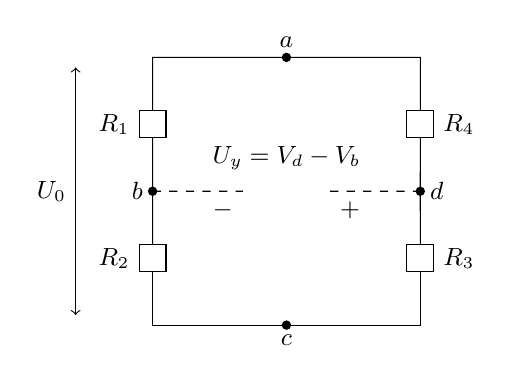
\begin{tikzpicture}[scale=.85, every node/.style={font=\small}]
\coordinate (a) at (0,4); \coordinate (b) at (-2,2);
\coordinate (c) at (0,0); \coordinate (d) at (2,2);
\draw (a) -- (-2,4) -- (-2,3.2);
\draw (-2.2,2.8) rectangle (-1.8,3.2);
\draw (-2,2.8) -- (b) -- (-2,1.2);
\draw (-2.2,.8) rectangle (-1.8,1.2);
\draw (-2,.8) -- (-2,0) -- (c);
\draw (a) -- (2,4) -- (2,3.2);
\draw (1.8,2.8) rectangle (2.2,3.2);
\draw (2,2.8) -- (d) -- (2,1.2);
\draw (1.8,.8) rectangle (2.2,1.2);
\draw (2,.8) -- (2,0) -- (c);
\draw[<->] (-3.15,.15) -- (-3.15,3.85) node[midway,left] {$U_0$};
\draw[dashed] (b) -- (-.65,2); \draw[dashed] (.65,2) -- (d);
\node at (-.95,1.72) {$-$}; \node at (.95,1.72) {$+$};
\node at (0,2.5) {$U_y=V_d-V_b$};
\foreach \p/\pos in {a/above,b/left,c/below,d/right} {\fill (\p) circle (2pt); \node[\pos] at (\p) {$\p$};}
\node[left] at (-2.2,3) {$R_1$}; \node[left] at (-2.2,1) {$R_2$};
\node[right] at (2.2,3) {$R_4$}; \node[right] at (2.2,1) {$R_3$};
\end{tikzpicture}
\end{center}

供桥电压为 $U_0=V_a-V_c$。下文默认电源内阻可忽略、输出端接高输入阻抗电路，因此桥路可按开路输出计算。两支路电流为
\[
I_{12}=\frac{U_0}{R_1+R_2},\qquad
I_{43}=\frac{U_0}{R_3+R_4}.
\]
由 $U_{ab}=I_{12}R_1$、$U_{ad}=I_{43}R_4$，得
\[
\boxed{U_y=U_0\left(\frac{R_1}{R_1+R_2}-\frac{R_4}{R_3+R_4}\right)
=U_0\frac{R_1R_3-R_2R_4}{(R_1+R_2)(R_3+R_4)}}.
\]

\dfn{电桥平衡}{输出 $U_y=0$ 时电桥平衡，条件为
\[
\boxed{R_1R_3=R_2R_4}.
\]
平衡条件只要求相应乘积相等，并不要求四个电阻一定相等。交换输出端，输出符号反转，平衡条件不变。}

\textbf{偏置法与归零法：}偏置法在初始平衡后由不平衡输出反映被测量；归零法在测量时调节已知桥臂，使输出重新为零，再由平衡关系求未知参量。前者适合连续动态测量，后者通过平衡判据测量参量。

\subsection{单臂、双臂与全桥：先看变化方向}

设初始四臂均为 $R$，工作后 $R_i=R(1+\delta_i)$，其中 $|\delta_i|\ll1$。对输出式在初始平衡点作一阶展开：
\[
\boxed{\frac{U_y}{U_0}\approx\frac14(\delta_1-\delta_2+\delta_3-\delta_4)}.
\]
因此，\textbf{相邻桥臂对输出的符号相反，对臂对输出的符号相同}。要使相邻有源桥臂的作用相加，应让其电阻等量反向变化；相邻臂等量同向变化则在理想情况下相互抵消。

令 $\delta=\Delta R/R=S_g\varepsilon$。$S_g$ 为应变片灵敏系数，应变 $\varepsilon$ 无量纲，$1\,\mu\varepsilon=10^{-6}$。典型接法如下。

\begin{table}[H]
\centering\small
\begin{tabularx}{\linewidth}{@{}p{1.5cm} p{4.25cm} X@{}}
\toprule
接法 & 有源桥臂的变化 & 输出与性质 \\
\midrule
单臂 & $R_1=R(1+\delta)$；其余不变 & $U_y=U_0\delta/(4+2\delta)\approx U_0\delta/4$。有桥路非线性。 \\
相邻双臂 & $R_1=R(1+\delta)$，$R_2=R(1-\delta)$；其余不变 & $U_y=U_0\delta/2$。等量反向条件下为精确线性。 \\
全桥 & $R_1,R_3=R(1+\delta)$，$R_2,R_4=R(1-\delta)$ & $U_y=U_0\delta$。四臂作用相加，为单臂小信号输出的4倍。 \\
\bottomrule
\end{tabularx}
\end{table}

双臂式的分母不变，因为 $R_1+R_2=2R$。全桥还利用了另一支路的反向分压变化。以上线性结论要求电阻变化\textbf{确实等量反向}；只有“两片”或“四片”这一数量信息，不能自动得到2倍或4倍灵敏度。若一个贴片只用作温度补偿而不承受机械应变，也不能把它按等量反向有源臂计算。

\dfn{电桥应变灵敏度}{直流供桥下，小信号零点灵敏度为
\[
K_\varepsilon=\left.\frac{\diff U_y}{\diff\varepsilon}\right|_{\varepsilon=0}
=\begin{cases}
U_0S_g/4,&\text{单臂},\\
U_0S_g/2,&\text{相邻等量反向双臂},\\
U_0S_g,&\text{等量交替变化全桥}.
\end{cases}
\]
这是电桥输出对应变的灵敏度，单位可写为 $\mathrm{V}/\text{应变}$；它与无量纲的应变片灵敏系数 $S_g$ 是不同概念。}

\subsection{温度补偿、供桥电压与测量误差}

\textbf{温度补偿利用和差特性。}相邻两片若具有相同温度系数、处在相同温度下，温升引起的等量同向阻值变化可相互抵消；若机械应变等量反向，则机械输出相加。补偿效果受贴片、温度分布、引线电阻和安装条件影响。

\textbf{提高 $U_0$ 会提高电压灵敏度，也会增大自热。}初始等臂桥中每臂承受 $U_0/2$，单臂耗散功率为 $U_0^2/(4R)$。供桥电压还会直接成比例影响输出，故电源稳定度也是测量精度的一部分。

\textbf{输出端负载不是总能忽略。}若接入有限输入电阻的仪表，输出电压要按桥路戴维南等效电阻与负载分压计算；初始等臂桥的输出等效电阻为 $R$。高输入阻抗放大器可减小这项误差。

\subsection{交流电桥：同时满足幅值与相位平衡}

交流供桥时，用复阻抗 $Z_i$ 替换电阻，输出相量满足相同形式：
\[
\underline U_y=\underline U_0\left(\frac{Z_1}{Z_1+Z_2}-\frac{Z_4}{Z_3+Z_4}\right),
\qquad \boxed{Z_1Z_3=Z_2Z_4}.
\]
若 $Z_i=|Z_i|e^{\iu\phi_i}$，平衡需同时满足
\[
|Z_1||Z_3|=|Z_2||Z_4|,\qquad
\phi_1+\phi_3=\phi_2+\phi_4\pmod{2\pi}.
\]
因此只调电阻未必能把交流输出调零，分布电容造成的相位分量也需要调节。例如取 $Z_1=R_1+1/(\iu\omega C_1)$、$Z_4=R_4+1/(\iu\omega C_4)$，$Z_2=R_2$、$Z_3=R_3$，分离实虚部得到
\[
R_1R_3=R_2R_4,\qquad \frac{R_3}{C_1}=\frac{R_2}{C_4}.
\]
若相应串联支路改为 $R_1+\iu\omega L_1$、$R_4+\iu\omega L_4$，则第二个条件为 $L_1R_3=L_4R_2$。交流电桥可测电阻、电感或电容变化；其精度还受频率稳定度、寄生参数和互感等影响。

\clearpage
\section{调制：把低频信息搬移到载波附近}
\label{sec:ch5-modulation}

\subsection{载波、调制信号与已调信号}
\noindent\keypoint{复习重点：频谱搬移发生在乘法中；边带间距由调制信号频率决定。}

\dfn{调制与解调}{设载波为 $c(t)=A_c\cos(2\pi f_ct+\phi_c)$。用被测信号 $x(t)$ 控制载波的幅值、瞬时频率或相位，分别称为调幅（AM）、调频（FM）和调相（PM）。从已调信号恢复 $x(t)$ 的过程称为解调。}

\textbf{为什么采用载波？}缓变或直流信号容易受放大器零点漂移影响；搬移到较高频段后，可用交流放大并通过带通环节抑制部分带外干扰。随后用已知参考把有效信息搬回基带。调制本身并不保证消除噪声，还需依据信号、干扰的频带及参考稳定度设计整条测量链。

先取单位余弦载波，抑制载波双边带调幅为
\[
x_a(t)=k_a x(t)\cos2\pi f_ct.
\]
沿用第2章 $X(f)=\int_{-\infty}^{\infty}x(t)e^{-\iu2\pi ft}\diff t$ 的变换约定，频谱为
\[
\boxed{X_a(f)=\frac{k_a}{2}\left[X(f-f_c)+X(f+f_c)\right]}.
\]
原谱分别向左右搬移 $f_c$ 并缩小为一半。若 $x(t)=M\cos2\pi f_mt$，积化和差给出
\[
x_a(t)=\frac{k_aM}{2}\cos2\pi(f_c+f_m)t
+\frac{k_aM}{2}\cos2\pi(f_c-f_m)t.
\]
当 $f_c>f_m>0$ 时，两条正频率边带在 $f_c\pm f_m$，每项的\textbf{时域峰值}是 $k_aM/2$；每条对应的\textbf{双边复谱线系数}还要再除以2。

若基带最高频率为 $f_m$，常取 $f_c>f_m$，使正、负载频附近的频谱分离；正载频一侧所占频带是 $[f_c-f_m,f_c+f_m]$，带宽为 $2f_m$。实际设计还需留出滤波器过渡带，并使载波比被测信号变化快得多。

\subsection{抑制载波与带载波调幅}

\begin{table}[H]
\centering\small
\begin{tabularx}{\linewidth}{@{}p{2.15cm} X X@{}}
\toprule
类型 & 表达式与频谱 & 包络和解调 \\
\midrule
抑制载波调幅 & $x_a=k_ax\cos\omega_ct$。若 $x$ 无直流，理想谱中无独立载波线。 & $x$ 可正可负；外轮廓反映 $|x|$，过零时载波反相。需相干参考恢复正负。 \\
带载波调幅 & $x_a=[D+k_ax]\cos\omega_ct$。$D$ 对应载频处的谱线。 & 若 $D+k_ax\geq0$，包络能保留 $D+k_ax$，检波后扣除偏置。 \\
\bottomrule
\end{tabularx}
\end{table}

对 $x=M\cos\omega_mt$、$D>0$，定义调幅度 $m_a=|k_aM|/D$。$m_a\leq1$ 时包络不翻折；$m_a>1$ 时出现过调，简单包络检波会丢失符号而失真。对多频信号，应检查实际极值或使用充分条件 $D\geq\max_t|k_ax(t)|$，不能只检查某一个谐波幅值。

\begin{center}
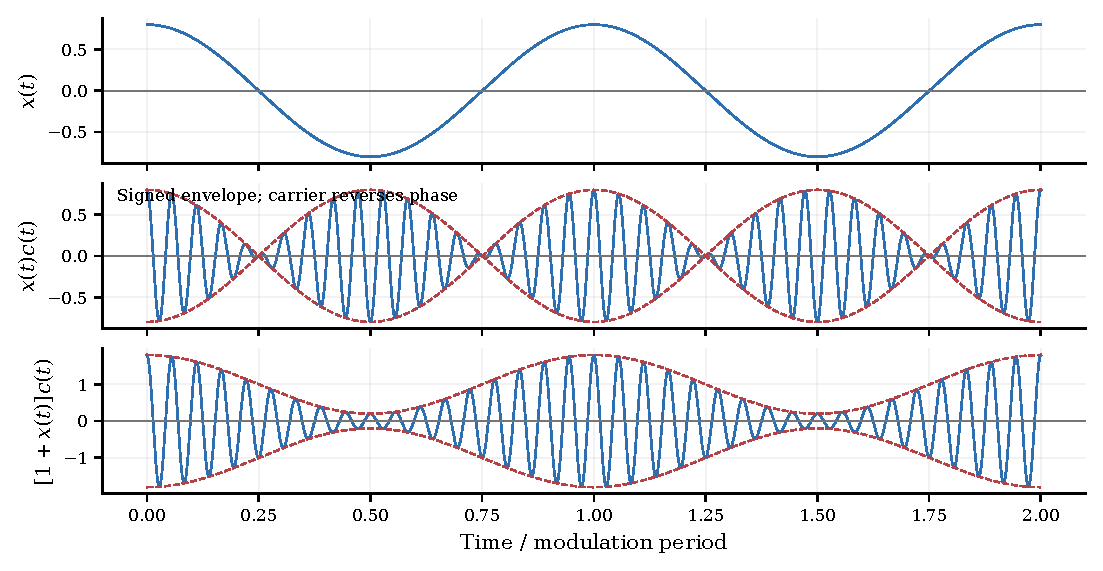
\includegraphics[width=.98\linewidth]{ch5-am-waveforms.pdf}
\end{center}
图中虚线显示有符号调制量及外轮廓。抑制载波的信号在 $x$ 变号时反相；加足够偏置后，外包络可以直接对应被测信号与偏置之和。

\subsection{交流电桥为什么能实现调幅}

若电阻应变片满足 $\Delta R/R=S_g\varepsilon(t)$，桥路系数记为 $k_b$，则
\[
u_y(t)=k_bS_g\varepsilon(t)u_0(t).
\]
单臂小信号取 $k_b=1/4$，等量反向双臂取 $1/2$，等量交替变化全桥取1。若 $u_0(t)=E\cos\omega_ct$，便得到
\[
\boxed{u_y(t)=k_bS_gE\varepsilon(t)\cos\omega_ct}.
\]
桥路既把应变转换为电压，又完成乘法调幅。应变为零时，理想平衡桥输出为零；应变变号时，输出相对激励的相位改变 $180^\circ$。因此动态应变测量通常需要能区分这两种相位的检波环节。

\clearpage
\section{解调：恢复幅值、波形与正负极性}
\label{sec:ch5-demodulation}

\subsection{同步乘法解调：低通留下基带}
\noindent\keypoint{复习重点：乘同频同相参考，再低通；乘法结果中的比例系数不能省略。}

对 $x_a(t)=k_ax(t)\cos\omega_ct$，与参考 $r(t)=B\cos(\omega_ct+\theta)$ 相乘：
\begin{align*}
v(t)&=k_aBx(t)\cos\omega_ct\cos(\omega_ct+\theta)\\
&=\frac{k_aB}{2}x(t)\cos\theta
+\frac{k_aB}{2}x(t)\cos(2\omega_ct+\theta).
\end{align*}
低通滤去 $2\omega_c$ 附近成分，得到
\[
\boxed{v_{\mathrm{LP}}(t)=\frac{k_aB}{2}\,x(t)\cos\theta}.
\]
参考同相时恢复信号比例为 $k_aB/2$；若希望输出恰为 $x(t)$，还需相应增益标定。相差 $90^\circ$ 时基带消失，相差 $180^\circ$ 时输出反号。若参考有频率偏差 $\Delta\omega$，基带会乘上 $\cos(\Delta\omega t+\theta)$，形成缓慢拍频，不能用固定标定系数补偿。

若 $x$ 占 $|f|\leq f_m$，二次乘法后的高频副本位于 $\pm2f_c$ 附近。理想低通截止频率可在
\[
f_m<f_{\mathrm{LP}}<2f_c-f_m
\]
之间选择；实际低通需在基带内满足幅相误差要求，并在高频副本前提供足够衰减。这里的 $f_{\mathrm{LP}}$ 不能机械取为 $f_m$，因为实际截止点通常已有明显衰减。

\subsection{包络检波：偏置足够才能保留波形}

对带载波信号 $x_a=[D+k_ax(t)]\cos\omega_ct$，若 $D+k_ax(t)\geq0$，理想包络与 $D+k_ax(t)$ 成比例，经低通平滑、扣除直流并标定增益，可恢复 $x(t)$。

若前面的括号可能为负，包络只能得到 $|D+k_ax(t)|$；正负部分发生折叠，后级线性滤波不能把丢失的符号重新找回。\textbf{抑制载波信号的普通整流检波一般不能恢复正负极性。}

在包络变化远慢于载波的条件下，可用整流平均理解检波增益。例如
\[
\overline{|\cos\omega_ct|}=\frac2\pi,
\]
故理想全波整流再平均的输出约为 $2|D+k_ax|/\pi$；二极管实际压降与RC充放电还会引入误差。包络检波器的时间常数需兼顾滤除载波纹波与跟随包络，常用定性条件为
\[
\frac1{\omega_c}\ll\tau_d\ll\frac1{\omega_m}.
\]
该式表达量级要求，实际设计还需按允许纹波与斜切失真确定。

\subsection{相敏检波：利用参考换向，保留极性}

相敏检波用与载波同步的参考控制换向。理想开关模型取
\[
q(t)=\sgn(\cos\omega_ct),\qquad x_a(t)=k_ax(t)\cos\omega_ct,
\]
则
\[
v(t)=x_a(t)q(t)=k_ax(t)|\cos\omega_ct|,
\qquad
\boxed{v_{\mathrm{LP}}(t)\approx\frac{2k_a}{\pi}x(t)}.
\]
当 $x>0$ 时换向后的平均值为正；当 $x<0$ 时平均值为负，因而能同时反映幅值与方向。这里的换向由\textbf{独立参考}控制，与把输入取绝对值的普通整流不同。

余弦绝对值的纹波基本重复频率是 $2f_c$，还含更高偶次成分；这说的是\textbf{检波纹波}，并非被测信号的所有频率都翻倍。低通后应保留原基带频率。开关相敏检波与正弦乘法解调的理想增益分别是 $2/\pi$ 与 $1/2$，使用哪一种模型，就按哪一种比例标定。

\begin{focusbox}{一条可解释的动态应变测量链}
稳定振荡器供桥 $\longrightarrow$ 交流电桥将应变调幅 $\longrightarrow$ 交流放大与载频附近选频 $\longrightarrow$ 用同源参考相敏检波 $\longrightarrow$ 低通恢复应变。

\textbf{要保留的有三项：}基带幅值、正负方向以及基带内的相对幅相关系。载波频率高，只说明信息搬移位置高，不代表被测应变一定变化得快。
\end{focusbox}

\subsection{调幅链可能产生的三种失真}

\begin{enumerate}
\item \textbf{频谱重叠：}载频太低，使搬移后的正负频谱副本相互覆盖，不能按独立边带分离。
\item \textbf{包络翻折：}带载波调幅偏置不足，包络检波丢失符号；这是特定解调方法造成的限制。
\item \textbf{传输幅相失真：}载波及各边带经过不同增益或相位变化，解调后的基带幅值关系或波形改变。放大器和带通环节应覆盖全部有效边带。
\end{enumerate}

\subsection{调频与调相：信息写入另一种载波参数}

对调频信号，瞬时频率定义为 $f_i(t)=f_c+k_fx(t)$，其中 $k_f$ 的单位为Hz/输入单位。由于频率是相位对时间的导数，\textbf{随时间变化的调频信号须积分得到相位}：
\[
\boxed{x_{\mathrm{FM}}(t)=A_c\cos\left[2\pi f_ct+
2\pi k_f\int_{t_0}^{t}x(\lambda)\diff\lambda+\phi_0\right]}.
\]
调相信号则可写为
\[
x_{\mathrm{PM}}(t)=A_c\cos[2\pi f_ct+k_px(t)+\phi_0].
\]
FM与PM保持理想幅值恒定。它们对某些幅值扰动可先限幅再解调，但频率、相位噪声仍会影响结果；所需带宽依赖频偏与输入频率，不能用固定倍数概括。

\textbf{传感中的调频：}若LC振荡器频率 $f=1/(2\pi\sqrt{LC})$，固定 $L$ 并让 $C$ 在 $C_0$ 附近微变，则
\[
\frac{\Delta f}{f_0}\approx-\frac12\frac{\Delta C}{C_0}.
\]
被测量引起的电容或电感变化因此可转为频率变化。鉴频可利用近似线性的频率--电压特性，或由周期、过零间隔计数等方法恢复信号。斜率鉴频先把频率变化转为幅值变化，再进行包络检波，要求频率偏移落在线性工作区内。

\clearpage
\section{滤波器：选择频带并控制幅相变化}
\label{sec:ch5-filters}

\subsection{四种选频特性与滤波的能力边界}
\noindent\keypoint{复习重点：先在频域分清有用成分与干扰，再确定通带和阻带。}

\dfn{滤波器}{滤波器是具有选频特性的系统，让目标频率成分按要求通过，并衰减其他频率成分。对LTI滤波器，
\[
Y(f)=H(\iu2\pi f)X(f).
\]
幅频特性决定每个成分的幅值变化，相频特性决定其相位变化。}

\begin{center}
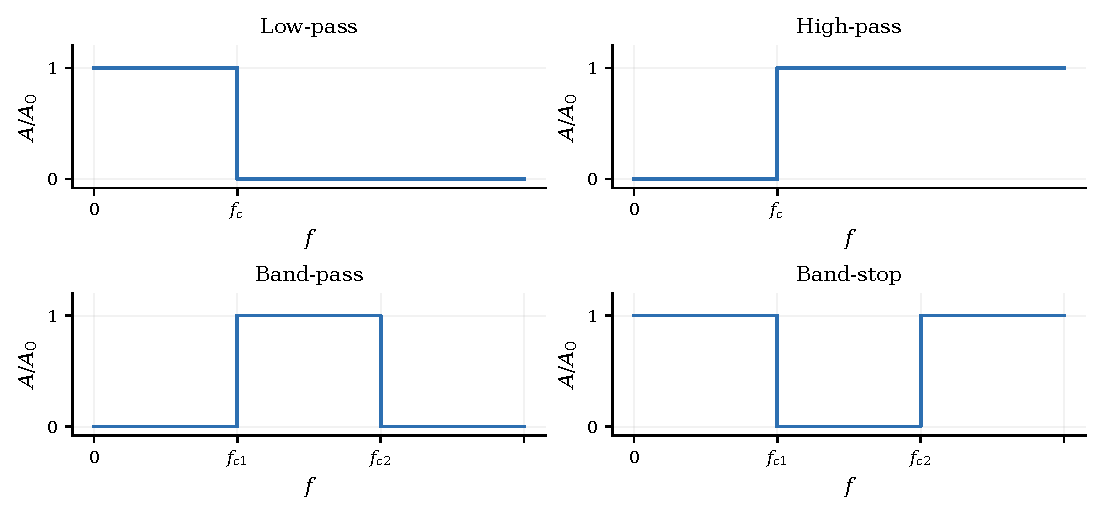
\includegraphics[width=.98\linewidth]{ch5-filter-types.pdf}
\end{center}

\begin{table}[H]
\centering\small
\begin{tabularx}{\linewidth}{@{}l p{3.6cm} X@{}}
\toprule
类型 & 正频率的主要通过范围 & 典型用途 \\
\midrule
低通 & $0\leq f<f_c$ & 解调后恢复基带；采样前限制带宽。 \\
高通 & $f>f_c$ & 去直流或缓慢漂移；保留较快变化。 \\
带通 & $f_{c1}<f<f_{c2}$ & 提取载频附近信号或某段振动。 \\
带阻 & 通过阻带以外的频率 & 抑制某段窄带干扰；很窄时常称陷波。 \\
\bottomrule
\end{tabularx}
\end{table}

实信号的频谱具有共轭对称性，图中只画正频率。若有效信号与干扰占同一频带，普通选频滤波会同时作用于二者，不能完全分离。即使频带不同，也应给实际滤波器留出过渡区域。

按实现形式，还可分为无源与有源、RC与LC、模拟与数字滤波器。有源电路可提供增益与缓冲；无源电路受级间阻抗影响；数字滤波在采样后处理数值序列。实现形式不同，选频与幅相分析的基本思想相通。

\subsection{理想滤波器与时间--频率折中}

理想低通在通带内满足不失真条件，通带外为零：
\[
H(f)=\begin{cases}
A_0e^{-\iu2\pi ft_0},&|f|<f_c,\\
0,&|f|>f_c.
\end{cases}
\]
它在通带内具有平坦幅值与线性相位。对应冲激响应为
\[
h(t)=2A_0f_c\Sa\!\left[2\pi f_c(t-t_0)\right],
\qquad \Sa u=\frac{\sin u}{u}.
\]
该响应向时间两侧无限延伸；任意有限 $t_0$ 下，$t<0$ 仍有非零响应，因此严格砖墙形低通不能由实时因果电路精确实现。

缩小带宽会拉宽冲激响应主瓣，滤波输出需要更长时间建立。以理想单位增益低通的阶跃响应为例，
\[
y(t)=\frac12+\frac1\pi\int_0^{2\pi f_c(t-t_0)}\frac{\sin u}{u}\diff u,
\]
按首次10\%至90\%交点定义的上升时间约为 $T_r\approx0.45/f_c$。这个系数随滤波器形状和时间指标而改变，不能把 $BT=\text{某固定数}$ 当作所有滤波器的定律。

\textbf{实际意义：}窄带有利于区分相近频率，却使时间响应变慢；宽带有利于跟踪快速变化，也会让更多带外邻近噪声进入。对瞬态和波形测量，除了幅值，还要检查相位或群延迟。

\subsection{实际滤波器的主要指标}

实际滤波器在通带与阻带之间存在过渡带，阻带也不会处处严格为零。设通带参考幅值为 $A_{\mathrm{ref}}$，归一化增益的分贝值定义为
\[
L_A(f)=20\log_{10}\frac{A(f)}{A_{\mathrm{ref}}}.
\]
按常用半功率约定，截止点满足
\[
\boxed{A(f_c)=\frac{A_{\mathrm{ref}}}{\sqrt2}},\qquad
L_A(f_c)=-10\log_{10}2\approx-3.0103\,\mathrm{dB}.
\]
这表示\textbf{相对于规定通带参考值下降约3 dB}，并不是绝对电压为 $-3\,\mathrm{dB}$；对同一阻抗上的功率，输出功率降为相应参考值的一半。

\begin{table}[H]
\centering\small
\begin{tabularx}{\linewidth}{@{}p{2.55cm} X@{}}
\toprule
指标 & 定义与解释 \\
\midrule
截止频率 & 按规定幅值限确定的通带边界；本文常用相对通带参考值的 $-3\,\mathrm{dB}$ 约定。 \\
带宽 & 带通的 $B=f_{c2}-f_{c1}$，单位为Hz；不能用两截止频率之比代替。 \\
中心频率 & 对数对称的带通频带取 $f_0=\sqrt{f_{c1}f_{c2}}$，是几何平均。 \\
品质因子 & $Q=f_0/B$，相对带宽为 $B/f_0=1/Q$；$Q$ 越大，频带相对越窄。 \\
通带纹波 & 通带内幅值相对参考值的起伏，须说明采用线性量还是分贝量。 \\
选择性 & 过渡带衰减的快慢，常用 $\mathrm{dB/oct}$ 或 $\mathrm{dB/dec}$ 表示。 \\
滤波器因数 & 常取 $\lambda=B_{-60\mathrm{dB}}/B_{-3\mathrm{dB}}$；采用同一参考，越接近1，裙边越陡。 \\
\bottomrule
\end{tabularx}
\end{table}

\nt{几何中心适用于本章的对数对称带通和倍频程分析。对任意不对称实际响应，应先说明中心频率的定义，不能把几何中心、算术中点和最大增益频率无条件等同。截止点也可能按其他指标规定，使用前须确认约定。}

\clearpage
\subsection{一阶RC低通与高通：幅值和相位一起计算}

令 $\tau=RC>0$，$q=\omega\tau=2\pi f\tau$。串联RC电路取电容两端为输出时是低通，取电阻两端为输出时是高通：
\begin{align*}
H_{\mathrm{LP}}(s)&=\frac1{1+\tau s},&
A_{\mathrm{LP}}&=\frac1{\sqrt{1+q^2}},&
\phi_{\mathrm{LP}}&=-\arctan q;\\
H_{\mathrm{HP}}(s)&=\frac{\tau s}{1+\tau s},&
A_{\mathrm{HP}}&=\frac{q}{\sqrt{1+q^2}},&
\phi_{\mathrm{HP}}&=\frac\pi2-\arctan q\quad(q>0).
\end{align*}
二者的转折频率都是
\[
\boxed{f_c=\frac1{2\pi RC}},\qquad \omega_c=\frac1{RC}.
\]
低通在转折点相位为 $-45^\circ$，高通为 $+45^\circ$。高通的输出超前输入；$q=0$ 时其幅值为零，相位按 $q\to0^+$ 的极限讨论。

\begin{center}
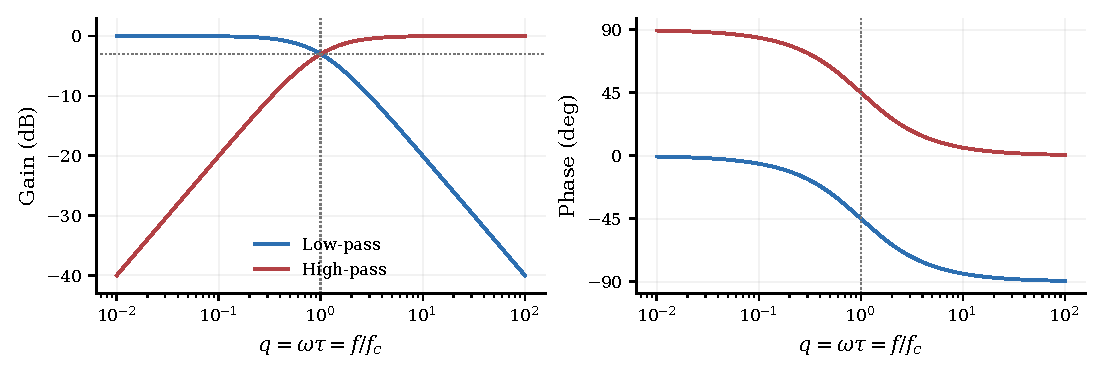
\includegraphics[width=.98\linewidth]{ch5-rc-frequency.pdf}
\end{center}
图中低通在高频端以约 $-20\,\mathrm{dB/dec}$（每频率加倍约 $-6\,\mathrm{dB}$）衰减，高通在低频端对应约 $+20\,\mathrm{dB/dec}$。渐近斜率描述远离转折点的趋势，不等于转折附近每个频率区间的精确变化。

\textbf{稳态输出的通用式：}若输入 $x_i(t)=X_i\cos(\omega_it+\theta_i)$，则
\[
y_i(t)=X_iA(\omega_i)\cos[\omega_it+\theta_i+\phi(\omega_i)].
\]
多频输入逐项计算再相加。滤波会保留各正弦分量的频率，但可改变它们的相对幅值和相位，因而改变叠加波形。

\subsection{串联与带通：复频响相乘，截止点重新检查}

在级间有缓冲或负载效应可忽略时，高通与低通串联可形成带通：
\[
H_{\mathrm{BP}}(s)=\frac{\tau_Hs}{1+\tau_Hs}\,\frac1{1+\tau_Ls},
\quad f_H=\frac1{2\pi\tau_H}<f_L=\frac1{2\pi\tau_L}.
\]
总幅值比为两级幅值比之积，总相位为两级相位之和。当两个转折频率相隔足够远，可把 $f_H$、$f_L$ 近似看作总带通的边界；接近时应由\textbf{总响应相对其通带参考值}重新求截止点。

类似地，$N$ 个相同一阶低通隔离串联，
\[
H_N(s)=(1+\tau s)^{-N},\qquad A_N(\omega)=[1+(\omega\tau)^2]^{-N/2}.
\]
令 $A_N=1/\sqrt2$ 得总体截止频率
\[
f_{c,N}=\frac{\sqrt{2^{1/N}-1}}{2\pi\tau}.
\]
串联使带外衰减更快，也会改变通带边界和相位；不能只把幅频曲线画得更陡而保持其他参数不变。并联相加时则须先把\textbf{复数频响}相加，再求模，不能直接相加两个幅值。

\subsection{恒带宽与恒带宽比滤波器组}

把信号同时送入多路带通滤波器，每路输出反映某段频带内的成分。若相邻频带在 $-3\,\mathrm{dB}$ 边界相接，应配合一致的增益标定，才能比较各通道输出。

\begin{center}
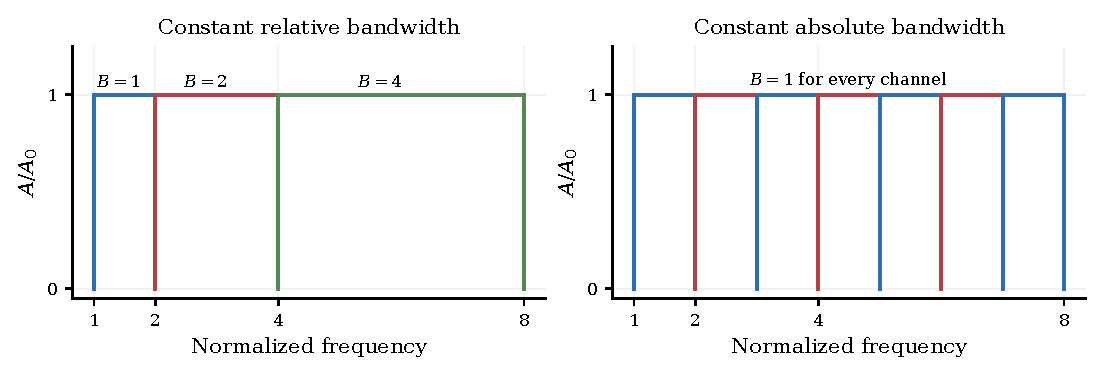
\includegraphics[width=.98\linewidth]{ch5-filter-bank.pdf}
\end{center}

\textbf{恒带宽：}各通道 $B$ 相同，具有相同的绝对频率分辨尺度；频带按线性频率分布，覆盖很宽频域时可能需要较多通道。

\textbf{恒带宽比：}各通道 $B/f_0$ 相同，亦即 $Q$ 相同；频率越高，绝对带宽越大，因此高频段区分固定Hz间隔的能力较弱，但保持相同的相对频率分辨尺度。

\dfn{倍频程与分数倍频程}{若上下截止频率之比为 $2^n$，该频带宽度为 $n$ 个倍频程：
\[
\boxed{\frac{f_{c2}}{f_{c1}}=2^n},\qquad
f_0=\sqrt{f_{c1}f_{c2}},\qquad
f_{c1}=2^{-n/2}f_0,\quad f_{c2}=2^{n/2}f_0.
\]
因此
\[
\boxed{\frac{B}{f_0}=2^{n/2}-2^{-n/2}},\qquad
Q=\frac1{2^{n/2}-2^{-n/2}}.
\]
完整一倍频程取 $n=1$，$1/3$ 倍频程取 $n=1/3$。}

\begin{table}[H]
\centering\small
\begin{tabular}{@{}c c c c@{}}
\toprule
频带宽度 & $f_{c2}/f_{c1}$ & $f_0/f_{c1}$ & $Q$ \\
\midrule
一倍频程 & $2$ & $\sqrt2$ & $\sqrt2\approx1.4142$ \\
$1/3$倍频程 & $2^{1/3}\approx1.2599$ & $2^{1/6}\approx1.1225$ & $\approx4.3185$ \\
\bottomrule
\end{tabular}
\end{table}
一倍频程的 $\sqrt2$ 是\textbf{中心频率与下限之比}，不是上、下限之比。若每路按相同 $n$ 衔接，相邻中心频率也满足 $f_{0,i+1}/f_{0,i}=2^n$。
